% !tex root = ../Thesis.tex

This literature review attempts to cover all the subjects relevant to pitch
correction. Music theory is investigated first, covering the topics of human
pitch perception and tuning. This section attempts to determine what it means for
pitch to be correct and how this relates to frequency. The idea is to get a list of
correct frequencies derived from a tuning system. After it is well known what
is musically considered to be a correct pitch, the general structure of how pitch
correction is approached is investigated. This structure naturally splits up into
modules and each of these modules is investigated further.

\section{Music Theory}

The intent of this section is to come up with a definition of what will be
considered correct pitch. Some foundational work is required to define basic
musical concepts in a rigorous way. To start we need to define exactly what is
meant by a musical note.

A note is a sound made from a musical instrument. It has a pitch, volume, timbre
and length. These are the characteristics a musician would consider when composing
a piece of music. Each of these characteristics have a more rigorous scientific
counterpart they are related to. Pitch relates to frequency; Volume relates to
amplitude; timbre relates to harmonic content and length relates to duration. The
characteristic pair relevant to pitch correction is the pitch and frequency pair
and needs to be covered in more depth.

\begin{wrapfigure}{L}{0.5\textwidth}
\includegraphics[width=0.5\textwidth,trim={3mm 0mm 20mm 8mm},clip]{Frequency-Vs-Pitch}
\caption{"Frequency vs Pitch"}
\label{fig:FrequencyVsPitch}
\end{wrapfigure}

Pitch and frequency are terms often used interchangeably but does not refer to the
same concept. Pitch is a \textit{sensation} experienced by humans when they hear
notes containing frequencies between 31Hz and 17.6 kHz\cite{Hearing}. The
sensation of pitch is scaled on an subjective ``high'' and ``low'' scale. The
higher the frequency, the higher the pitch perceived and the lower the frequency,
the lower the pitch perceived. This relationship between pitch and frequency is
generally considered to be logarithmic. Slight deviations from the expected
logarithmic relationship was found\cite{PitchVsFrequency} but was deemed minor
and unnecessary to incorporate for this project.

In Figure \ref{fig:FrequencyVsPitch} the relationship of frequency and pitch is
shown. Pitch is generally denoted by letters ranging from A to G with
sharps(\musSharp) and flats(\musFlat) called accidentals.  This is due to a long
history of convention and is irrelevant for now. The main takeaway is that the
perceived change in pitch is constant for each successive note. From this graph it
can be seen that frequency is exponentially dependent on pitch, or inversely,
pitch is logarithmically dependent on frequency.

From Figure \ref{fig:FrequencyVsPitch} a list of correct frequencies is obtained.
The method by which this list is obtained, originates from a concept called pitch
harmony. Two notes sounds good or in tune if their frequencies produce a simple
ratio\cite{Harmony}. For example an octave produces a ratio of 1:2 and a perfect
5th produces a ratio of 3:2. Figure \ref{fig:Harmony} shows how these two
harmonies are seen when their waveforms are plotted. The superposition created by
the two notes creating the interval has a short repeating pattern. The fact that
this pattern is short corresponds to the property of a simple ratio of
frequencies.  This short pattern/simple ratio is the origin of why two notes sound
harmonious.

\begin{figure}[h]
\centering
{\bf Octave Interval}
\begin{tabular}{c c c}
	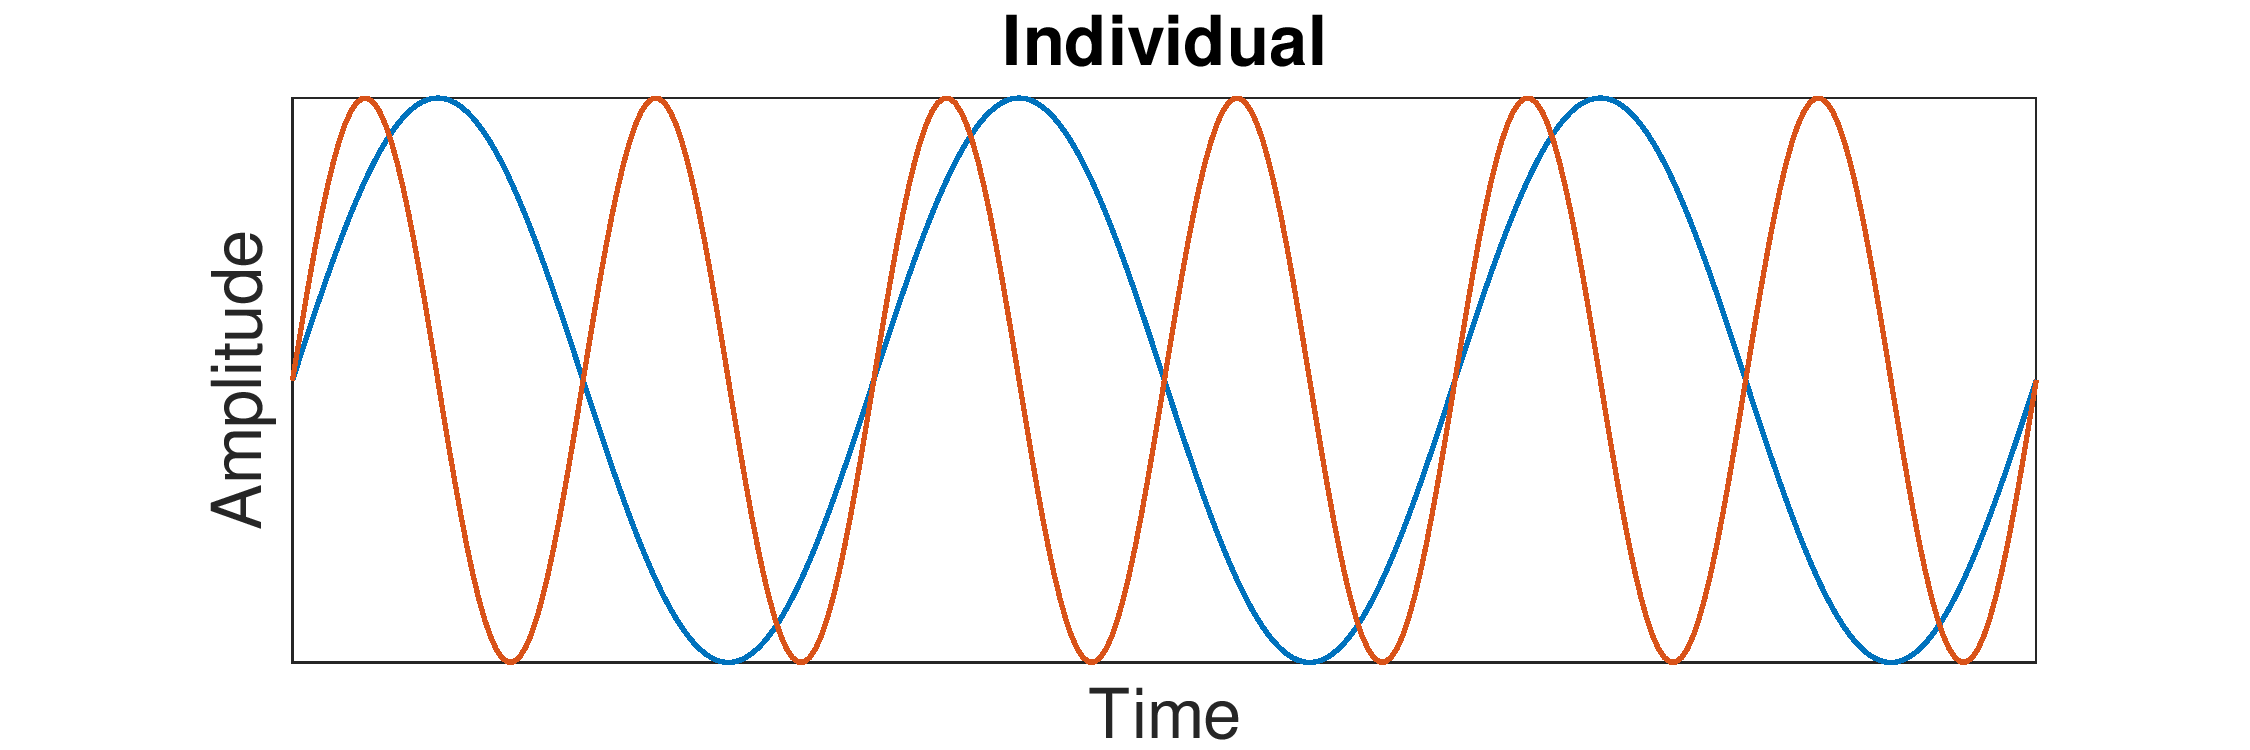
\includegraphics[align=c, width=0.4\textwidth,
		trim={3.5cm 0 3.5cm 0},clip]
		{HarmonyOctaveSeparate}

	& \huge$\rightarrow$ &
	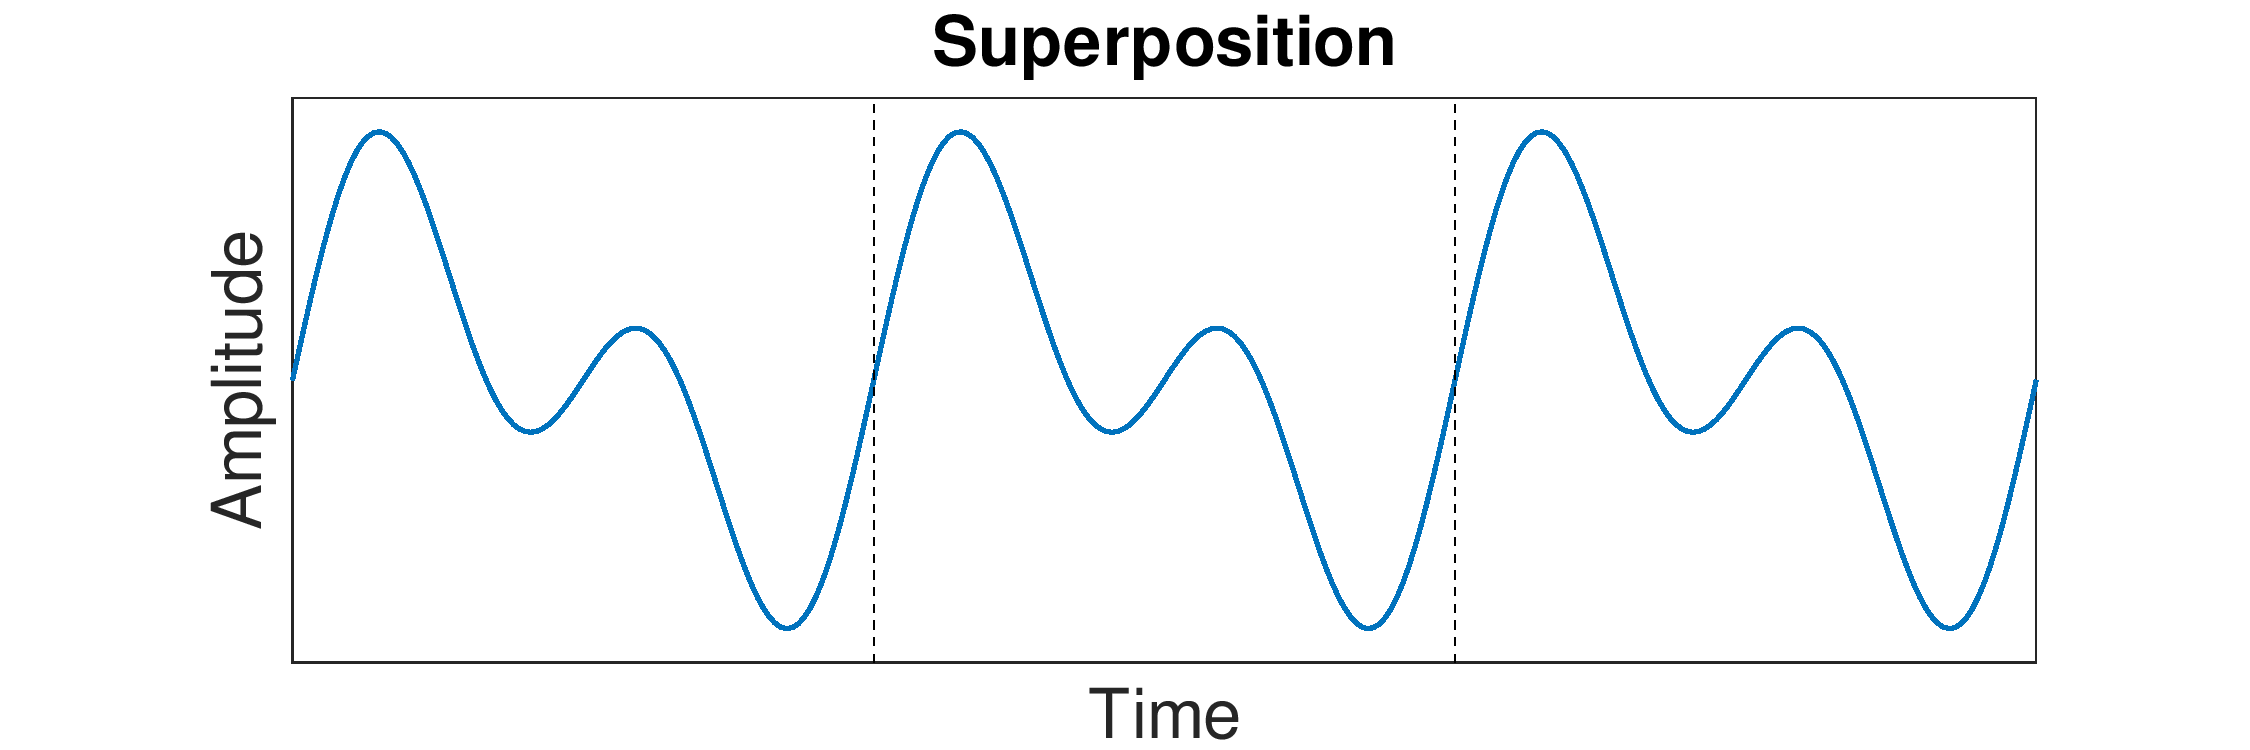
\includegraphics[align=c, width=0.4\textwidth,
		trim={3.5cm 0 3.5cm 0},clip]
		{HarmonyOctaveSuper}\\
\end{tabular}

\centering

{\bf Fifth Interval}
\begin{tabular}{c c c}
	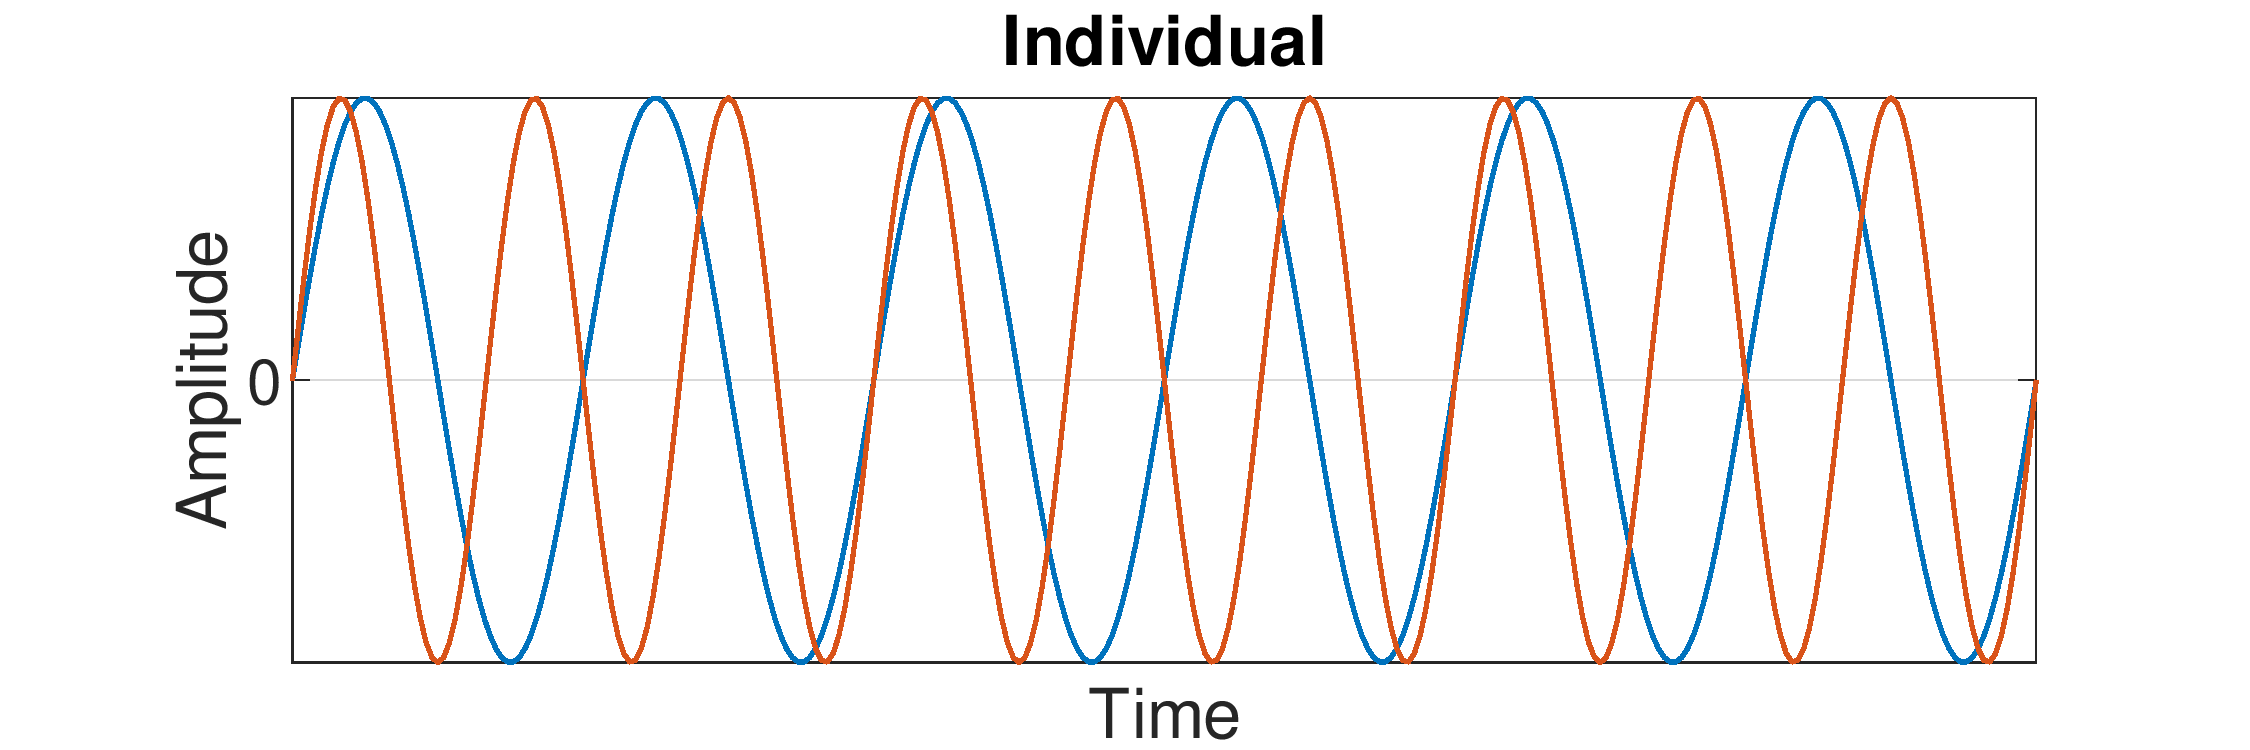
\includegraphics[align=c, width=0.4\textwidth,
		trim={3.5cm 0 3.5cm 0},clip]
		{HarmonyFifthSeparate}
	& \huge$\rightarrow$ &
	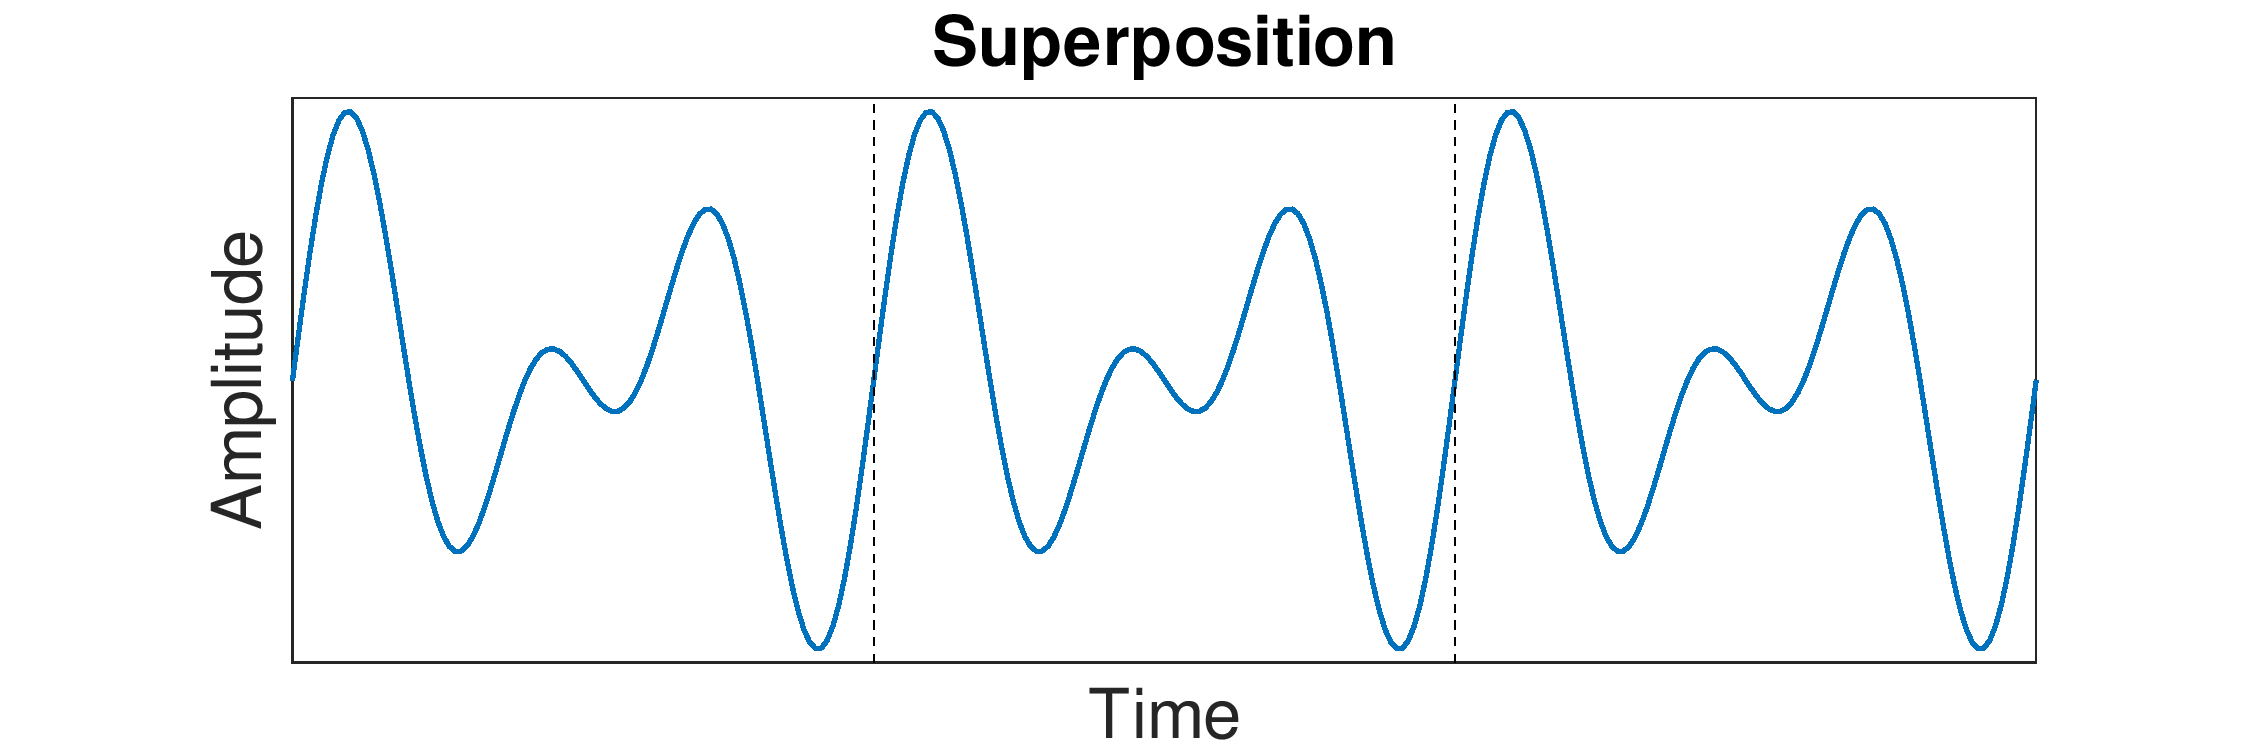
\includegraphics[align=c, width=0.4\textwidth,
		trim={3.5cm 0 3.5cm 0},clip]
		{HarmonyFifthSuper}\\
\end{tabular}
\caption{Harmonic interference of two intervals}
\label{fig:Harmony}
\end{figure}

This concept of harmony gives a simple method to start creating a list of
frequencies that would sound good together. This list is created by starting with
an arbitrary frequency (440 Hz) and using these simple harmonic ratio's to create
a scale. In table \ref{tab:JustTuning} a list of these ratio's and corresponding
interval names are given. This is referred to as {\it just tuning}. This tuning
method was naturally discovered because it corresponds to the different modes by
which a string vibrates when plucked\cite{StringVibrate}.

\begin{table}[h]
\centering
\caption{Interval Names and Ratio's of Just Tuning}
\begin{tabu} to \textwidth { | X[l] | X[c] | X[r] | }
	\hline \bf Interval Name & \bf Ratio  & Frequency Relative to 55 Hz \\
	\hline
\end{tabu}
\label{tab:JustTuning}
\end{table}

\color{red}
To do:
\begin{itemize}
	\item Complete table
\end{itemize}
\color{black}

\noindent Unfortunately this just tuning method posed a problem when harpsichords
and clavichords (piano-like instruments) were introduced. These instruments
required to be in tune for any starting note. For a tuning system to allow this,
an interval is required that touches all the wanted intervals when consecutively
applied. Since pitch is logarithmically dependent on frequency, we require a
single real number $r$ raised to the power of some arbitrary integer n so that the
result equals all the desired interval ratios.  Mathematically we require:

\begin{equation}\label{GeneralRationalTheorem}
	\exists r \in \mathbb{R} \text{ s.t. } R \subseteq \{ r^n | n \in \mathbb{N} \}
	\text{ where } R = \{ \frac{2}{1}, \frac{3}{2}, \dots \}
\end{equation}

\noindent This in not possible, as shown in Equation \ref{eq:mine}. The best one
can do is choose which interval you want to keep consistent accross all starting
notes and choose a sufficiently small sub-division so that each the note is close
enough to it's wanted harmonic ratio that it is imperceptable to the listener.
This is exactly what equal tempered tuning does. The interval kept constant is the
octave and it is divided into 12 sub-intervals called semitones. Table
\ref{table:EqualTemper} shows the modern equal tempered tuning ratios and their
related interval names. For all western scales a subset of these frequencies are
taken to produce the desired scale.

\color{red}
To do:
\begin{itemize}
	\item Show equal tempered tuning vs just interval graph
	\item Tie back to the fact that this gives us a definition of correct
\end{itemize}
\color{black}

\section{General Pitch Correction Structure}

\color{red}
To Do:
\begin{itemize}
	\item Stages and sections needed e.g.:
	\begin{itemize}
		\item Segmentation/Windowing
		\item Frequency detection
		\item Decide where to shift
		\item Frequency scaling
	\end{itemize}
	\item Add a flow diagram
\end{itemize}
\color{black}

\section{Segmentation}

\color{red}
To do:
\begin{itemize}
	\item Describe what segmentation is and why it is necessary
	\item Describe stages
	\begin{itemize}
		\item Split (overlap)
		\item Do computation
		\item Stitch (overlap and add)
	\end{itemize}
	\item Reason to overlap and size of overlapping (TRADE-OFF)
	\item Window size (TRADE-OFF)
	\begin{itemize}
		\item Small means low resolution
		\item Large means latency
		\item Small generally means more computation
	\end{itemize}
	\item Properties to preserve relevant to real time auto tuning
\end{itemize}
\color{black}

\section{Frequency Detection}

\color{red}
To do:
\begin{itemize}
	\item Explain that there is no single go-to method
	\item Different methods have different characteristics
	\item What is important for this application
	\item Give overview of which methods will be investigated
\end{itemize}
\color{black}

\subsection{Zero Crossing Method}

\color{red}
To do:
\begin{itemize}
	\item Describe method roughly
	\item More in depth description comes in implementation section
\end{itemize}
\color{black}

\subsection{Periodogram Method}

\color{red}
To do:
\begin{itemize}
	\item Describe method roughly
	\item More in depth description comes in implementation section
\end{itemize}
\color{black}

\subsection{Max FFT Method}

\color{red}
To do:
\begin{itemize}
	\item Describe method roughly
	\item More in depth description comes in implementation section
\end{itemize}
\color{black}

\subsection{YIN's Method}

\color{red}
To do:
\begin{itemize}
	\item Describe method roughly
	\item More in depth description comes in implementation section
\end{itemize}
\color{black}

\section{Frequency Scaling}

\color{red}
To do:
\begin{itemize}
	\item General approach is to expand/extrapolate frequency
	\item Time domain approaches and frequency domain approaches
	\item Introduce two approaches Phase Vocoder and pitch synchronous overlap and add
\end{itemize}
\color{black}

\subsection{Phase Vocoder}

\color{red}
To do:
\begin{itemize}
	\item Describe method roughly
	\item More in depth description comes in implementation section
\end{itemize}
\color{black}

\subsection{PSOLA}

\color{red}
To do:
\begin{itemize}
	\item Describe method roughly
	\item More in depth description comes in implementation section
\end{itemize}
\color{black}
